\documentclass[twoside]{book}

% Packages required by doxygen
\usepackage{calc}
\usepackage{doxygen}
\usepackage{graphicx}
\usepackage[utf8]{inputenc}
\usepackage{makeidx}
\usepackage{multicol}
\usepackage{multirow}
\usepackage{textcomp}
\usepackage[table]{xcolor}

% Font selection
\usepackage[T1]{fontenc}
\usepackage{mathptmx}
\usepackage[scaled=.90]{helvet}
\usepackage{courier}
\usepackage{amssymb}
\usepackage{sectsty}
\renewcommand{\familydefault}{\sfdefault}
\allsectionsfont{%
  \fontseries{bc}\selectfont%
  \color{darkgray}%
}
\renewcommand{\DoxyLabelFont}{%
  \fontseries{bc}\selectfont%
  \color{darkgray}%
}

% Page & text layout
\usepackage{geometry}
\geometry{%
  a4paper,%
  top=2.5cm,%
  bottom=2.5cm,%
  left=2.5cm,%
  right=2.5cm%
}
\tolerance=750
\hfuzz=15pt
\hbadness=750
\setlength{\emergencystretch}{15pt}
\setlength{\parindent}{0cm}
\setlength{\parskip}{0.2cm}
\makeatletter
\renewcommand{\paragraph}{%
  \@startsection{paragraph}{4}{0ex}{-1.0ex}{1.0ex}{%
    \normalfont\normalsize\bfseries\SS@parafont%
  }%
}
\renewcommand{\subparagraph}{%
  \@startsection{subparagraph}{5}{0ex}{-1.0ex}{1.0ex}{%
    \normalfont\normalsize\bfseries\SS@subparafont%
  }%
}
\makeatother

% Headers & footers
\usepackage{fancyhdr}
\pagestyle{fancyplain}
\fancyhead[LE]{\fancyplain{}{\bfseries\thepage}}
\fancyhead[CE]{\fancyplain{}{}}
\fancyhead[RE]{\fancyplain{}{\bfseries\leftmark}}
\fancyhead[LO]{\fancyplain{}{\bfseries\rightmark}}
\fancyhead[CO]{\fancyplain{}{}}
\fancyhead[RO]{\fancyplain{}{\bfseries\thepage}}
\fancyfoot[LE]{\fancyplain{}{}}
\fancyfoot[CE]{\fancyplain{}{}}
\fancyfoot[RE]{\fancyplain{}{\bfseries\scriptsize Generated on Tue Apr 14 2015 03\-:23\-:27 for D\-N\-S\-Analyser by Doxygen }}
\fancyfoot[LO]{\fancyplain{}{\bfseries\scriptsize Generated on Tue Apr 14 2015 03\-:23\-:27 for D\-N\-S\-Analyser by Doxygen }}
\fancyfoot[CO]{\fancyplain{}{}}
\fancyfoot[RO]{\fancyplain{}{}}
\renewcommand{\footrulewidth}{0.4pt}
\renewcommand{\chaptermark}[1]{%
  \markboth{#1}{}%
}
\renewcommand{\sectionmark}[1]{%
  \markright{\thesection\ #1}%
}

% Indices & bibliography
\usepackage{natbib}
\usepackage[titles]{tocloft}
\setcounter{tocdepth}{3}
\setcounter{secnumdepth}{5}
\makeindex

% Hyperlinks (required, but should be loaded last)
\usepackage{ifpdf}
\ifpdf
  \usepackage[pdftex,pagebackref=true]{hyperref}
\else
  \usepackage[ps2pdf,pagebackref=true]{hyperref}
\fi
\hypersetup{%
  colorlinks=true,%
  linkcolor=blue,%
  citecolor=blue,%
  unicode%
}

% Custom commands
\newcommand{\clearemptydoublepage}{%
  \newpage{\pagestyle{empty}\cleardoublepage}%
}


%===== C O N T E N T S =====

\begin{document}

% Titlepage & ToC
\hypersetup{pageanchor=false}
\pagenumbering{roman}
\begin{titlepage}
\vspace*{7cm}
\begin{center}%
{\Large D\-N\-S\-Analyser }\\
\vspace*{1cm}
{\large Generated by Doxygen 1.8.6}\\
\vspace*{0.5cm}
{\small Tue Apr 14 2015 03:23:27}\\
\end{center}
\end{titlepage}
\clearemptydoublepage
\tableofcontents
\clearemptydoublepage
\pagenumbering{arabic}
\hypersetup{pageanchor=true}

%--- Begin generated contents ---
\chapter{Hierarchical Index}
\section{Class Hierarchy}
This inheritance list is sorted roughly, but not completely, alphabetically\-:\begin{DoxyCompactList}
\item \contentsline{section}{Activity}{\pageref{class_activity}}{}
\item \contentsline{section}{Convert}{\pageref{class_convert}}{}
\item \contentsline{section}{D\-B\-Connection}{\pageref{class_d_b_connection}}{}
\item \contentsline{section}{D\-N\-S\-Wrapper}{\pageref{class_d_n_s_wrapper}}{}
\item \contentsline{section}{Payload\-Retriever}{\pageref{class_payload_retriever}}{}
\item \contentsline{section}{Pcap\-Reader}{\pageref{class_pcap_reader}}{}
\item \contentsline{section}{Protocol\-State\-Machine}{\pageref{class_protocol_state_machine}}{}
\item \contentsline{section}{State}{\pageref{class_state}}{}
\item \contentsline{section}{Transition\-Support}{\pageref{class_transition_support}}{}
\item Hash\-Map\begin{DoxyCompactList}
\item \contentsline{section}{Hasher}{\pageref{class_hasher}}{}
\end{DoxyCompactList}
\item Observable\begin{DoxyCompactList}
\item \contentsline{section}{Event}{\pageref{class_event}}{}
\item \contentsline{section}{State\-Machine}{\pageref{class_state_machine}}{}
\end{DoxyCompactList}
\item Observer\begin{DoxyCompactList}
\item \contentsline{section}{Transition}{\pageref{class_transition}}{}
\end{DoxyCompactList}
\item Pcap\-Packet\begin{DoxyCompactList}
\item \contentsline{section}{Packet}{\pageref{class_packet}}{}
\end{DoxyCompactList}
\item Serializable\begin{DoxyCompactList}
\item \contentsline{section}{Packet}{\pageref{class_packet}}{}
\end{DoxyCompactList}
\end{DoxyCompactList}

\chapter{Class Index}
\section{Class List}
Here are the classes, structs, unions and interfaces with brief descriptions\-:\begin{DoxyCompactList}
\item\contentsline{section}{\hyperlink{class_activity}{Activity} }{\pageref{class_activity}}{}
\item\contentsline{section}{\hyperlink{class_convert}{Convert} }{\pageref{class_convert}}{}
\item\contentsline{section}{\hyperlink{class_d_b_connection}{D\-B\-Connection} }{\pageref{class_d_b_connection}}{}
\item\contentsline{section}{\hyperlink{class_d_n_s_wrapper}{D\-N\-S\-Wrapper} }{\pageref{class_d_n_s_wrapper}}{}
\item\contentsline{section}{\hyperlink{class_event}{Event} }{\pageref{class_event}}{}
\item\contentsline{section}{\hyperlink{class_hasher}{Hasher} }{\pageref{class_hasher}}{}
\item\contentsline{section}{\hyperlink{class_packet}{Packet} }{\pageref{class_packet}}{}
\item\contentsline{section}{\hyperlink{class_payload_retriever}{Payload\-Retriever} }{\pageref{class_payload_retriever}}{}
\item\contentsline{section}{\hyperlink{class_pcap_reader}{Pcap\-Reader} }{\pageref{class_pcap_reader}}{}
\item\contentsline{section}{\hyperlink{class_protocol_state_machine}{Protocol\-State\-Machine} }{\pageref{class_protocol_state_machine}}{}
\item\contentsline{section}{\hyperlink{class_state}{State} }{\pageref{class_state}}{}
\item\contentsline{section}{\hyperlink{class_state_machine}{State\-Machine} }{\pageref{class_state_machine}}{}
\item\contentsline{section}{\hyperlink{class_transition}{Transition} }{\pageref{class_transition}}{}
\item\contentsline{section}{\hyperlink{class_transition_support}{Transition\-Support} }{\pageref{class_transition_support}}{}
\end{DoxyCompactList}

\chapter{Class Documentation}
\hypertarget{class_activity}{\section{Activity Class Reference}
\label{class_activity}\index{Activity@{Activity}}
}
\subsection*{Public Member Functions}
\begin{DoxyCompactItemize}
\item 
\hypertarget{class_activity_a1ecc6ee41881e5ffa81356f086b6ccc4}{void {\bfseries Entry\-Action\-Init} ()}\label{class_activity_a1ecc6ee41881e5ffa81356f086b6ccc4}

\item 
\hypertarget{class_activity_aa61692846e34219d956f7d8e460682ac}{void {\bfseries Exit\-Action\-Init} ()}\label{class_activity_aa61692846e34219d956f7d8e460682ac}

\item 
\hypertarget{class_activity_a43f600dfb966a5aec048dbad2552064b}{void {\bfseries next\-State\-Init} (\hyperlink{class_state_machine}{State\-Machine} S\-M)}\label{class_activity_a43f600dfb966a5aec048dbad2552064b}

\item 
\hypertarget{class_activity_aa6746c91dc931e7df308171bb12db7cb}{void {\bfseries Entry\-Action\-A} ()}\label{class_activity_aa6746c91dc931e7df308171bb12db7cb}

\item 
\hypertarget{class_activity_a50975cab4cfcb2f1ab2cdc9795bddfa3}{void {\bfseries next\-State\-A} (\hyperlink{class_state_machine}{State\-Machine} S\-M)}\label{class_activity_a50975cab4cfcb2f1ab2cdc9795bddfa3}

\item 
\hypertarget{class_activity_a85bb3354e0c4ceab6e942f7ed1a6c581}{void {\bfseries Exit\-Action\-A} ()}\label{class_activity_a85bb3354e0c4ceab6e942f7ed1a6c581}

\item 
\hypertarget{class_activity_ace37aec6b652bcfb415dac80c59f06d6}{void {\bfseries Entry\-Action\-B} ()}\label{class_activity_ace37aec6b652bcfb415dac80c59f06d6}

\item 
\hypertarget{class_activity_a3adc646b4161d2e62aa386df5c630319}{void {\bfseries next\-State\-B} (\hyperlink{class_state_machine}{State\-Machine} S\-M)}\label{class_activity_a3adc646b4161d2e62aa386df5c630319}

\item 
\hypertarget{class_activity_aa921effecbc8143694e3de07df0a0859}{void {\bfseries Exit\-Action\-B} ()}\label{class_activity_aa921effecbc8143694e3de07df0a0859}

\item 
\hypertarget{class_activity_ae4d12cc83fca914c5cdfe1ab69907556}{void {\bfseries Entry\-Action\-C} ()}\label{class_activity_ae4d12cc83fca914c5cdfe1ab69907556}

\item 
\hypertarget{class_activity_a51bc3f0f75d7eab7cb82c2ded79d0903}{void {\bfseries next\-State\-C} (\hyperlink{class_state_machine}{State\-Machine} S\-M)}\label{class_activity_a51bc3f0f75d7eab7cb82c2ded79d0903}

\item 
\hypertarget{class_activity_a438a754b7b8ca9e6492b04e26b6a4922}{void {\bfseries Exit\-Action\-C} ()}\label{class_activity_a438a754b7b8ca9e6492b04e26b6a4922}

\item 
\hypertarget{class_activity_a2eeed6fd49bd8807fc278a9744f9f1ba}{void {\bfseries Entry\-Action\-D} ()}\label{class_activity_a2eeed6fd49bd8807fc278a9744f9f1ba}

\item 
\hypertarget{class_activity_a109b514b15a9da22e1f6f70ab3d2913a}{void {\bfseries next\-State\-D} (\hyperlink{class_state_machine}{State\-Machine} S\-M)}\label{class_activity_a109b514b15a9da22e1f6f70ab3d2913a}

\item 
\hypertarget{class_activity_a09817f352494f36a479112ab94122058}{void {\bfseries Exit\-Action\-D} ()}\label{class_activity_a09817f352494f36a479112ab94122058}

\item 
\hypertarget{class_activity_a760d77b12bcba496fee34ee19817cc35}{void {\bfseries Entry\-Action\-E} ()}\label{class_activity_a760d77b12bcba496fee34ee19817cc35}

\item 
\hypertarget{class_activity_a09a088c9d6b3e9e60b60c131ef37b9fd}{void {\bfseries next\-State\-E} (\hyperlink{class_state_machine}{State\-Machine} S\-M)}\label{class_activity_a09a088c9d6b3e9e60b60c131ef37b9fd}

\item 
\hypertarget{class_activity_a656bf04826d55c2e804593658677980b}{void {\bfseries Exit\-Action\-E} ()}\label{class_activity_a656bf04826d55c2e804593658677980b}

\item 
\hypertarget{class_activity_a08603ceaa5de05471bdde9d7ba280166}{void {\bfseries Entry\-Action\-End} ()}\label{class_activity_a08603ceaa5de05471bdde9d7ba280166}

\item 
\hypertarget{class_activity_ae1eab2fa03abfe99dc03050f63c3b584}{void {\bfseries Exit\-Action\-End} ()}\label{class_activity_ae1eab2fa03abfe99dc03050f63c3b584}

\item 
\hypertarget{class_activity_ad7a208274460ca5febd5cd5c2ecd0151}{void {\bfseries next\-State\-End} (\hyperlink{class_state_machine}{State\-Machine} S\-M)}\label{class_activity_ad7a208274460ca5febd5cd5c2ecd0151}

\end{DoxyCompactItemize}


The documentation for this class was generated from the following file\-:\begin{DoxyCompactItemize}
\item 
src/Activity.\-java\end{DoxyCompactItemize}

\hypertarget{class_convert}{\section{Convert Class Reference}
\label{class_convert}\index{Convert@{Convert}}
}
\subsection*{Static Public Member Functions}
\begin{DoxyCompactItemize}
\item 
\hypertarget{class_convert_aebce018f64c3710e0f125ba3d5c5b0e7}{static byte\mbox{[}$\,$\mbox{]} {\bfseries to\-Byte\-Array} (Object o)}\label{class_convert_aebce018f64c3710e0f125ba3d5c5b0e7}

\item 
\hypertarget{class_convert_a7f2014d77c433c9097ce93061318d515}{static Object {\bfseries to\-Object} (byte\mbox{[}$\,$\mbox{]} bytes)}\label{class_convert_a7f2014d77c433c9097ce93061318d515}

\item 
\hypertarget{class_convert_aae1b0b913419b9507a83865ecd67864e}{static String {\bfseries to\-Hex} (byte\mbox{[}$\,$\mbox{]} bytes)}\label{class_convert_aae1b0b913419b9507a83865ecd67864e}

\item 
\hypertarget{class_convert_a4e74cdecb76c72ec0cc2e9af812275ab}{static String {\bfseries to\-Binary\-String} (byte\mbox{[}$\,$\mbox{]} bytes)}\label{class_convert_a4e74cdecb76c72ec0cc2e9af812275ab}

\item 
\hypertarget{class_convert_ab26526aaf2b8e31847f9a2d1aa41492a}{static String {\bfseries to\-Binary\-String} (byte bytes)}\label{class_convert_ab26526aaf2b8e31847f9a2d1aa41492a}

\item 
\hypertarget{class_convert_a4024fa392652d521ada3ae32805cc2fb}{static String {\bfseries to\-Hex} (String bytes)}\label{class_convert_a4024fa392652d521ada3ae32805cc2fb}

\item 
\hypertarget{class_convert_af3b7a4f9fe63d11156958117a3f1d246}{static void {\bfseries main} (String\mbox{[}$\,$\mbox{]} args)}\label{class_convert_af3b7a4f9fe63d11156958117a3f1d246}

\end{DoxyCompactItemize}


The documentation for this class was generated from the following file\-:\begin{DoxyCompactItemize}
\item 
src/Convert.\-java\end{DoxyCompactItemize}

\hypertarget{class_d_b_connection}{\section{D\-B\-Connection Class Reference}
\label{class_d_b_connection}\index{D\-B\-Connection@{D\-B\-Connection}}
}
\subsection*{Public Member Functions}
\begin{DoxyCompactItemize}
\item 
String \hyperlink{class_d_b_connection_a5db915c711a7fe87b76839db531b045a}{get\-D\-B\-Name} ()
\item 
Connection \hyperlink{class_d_b_connection_ad931f04e763064e0783ac6b812e71380}{get\-Connect} ()
\item 
void \hyperlink{class_d_b_connection_ac3c0a6e8676f9b4e4197088c3a2cee2b}{set\-Properties} ()
\item 
Connection \hyperlink{class_d_b_connection_abf660ee4c1d0c01371b9aaebb95bffda}{get\-Connection} ()
\item 
void \hyperlink{class_d_b_connection_a9ff0b2dbf7570e376582d966c631aefb}{create\-Schema} (String schemaname)  throws S\-Q\-L\-Exception
\item 
void \hyperlink{class_d_b_connection_a04648cfe383fc86dab0b7c89040cc2a3}{drop\-Table} (String table\-Name)  throws S\-Q\-L\-Exception
\item 
void \hyperlink{class_d_b_connection_a52ec5e8f563ccab29045a874d5727ac6}{create\-Table} (String table\-Name, String columns)  throws S\-Q\-L\-Exception 
\item 
void \hyperlink{class_d_b_connection_a7df51ca3564584b74dd970c1b0fa06fe}{populate\-Table} (String table\-Name, Object...\-parameters)  throws S\-Q\-L\-Exception 
\item 
Result\-Set \hyperlink{class_d_b_connection_ae45cfcbf6f06447c03a32fddb75f3b4e}{retrieve\-Result\-Set} (String table\-Name, String columns, String conditions)  throws S\-Q\-L\-Exception 
\end{DoxyCompactItemize}


\subsection{Detailed Description}
This class creates connections to the database by taking the required parameters in constructor. \begin{DoxyAuthor}{Author}
amit 
\end{DoxyAuthor}


\subsection{Member Function Documentation}
\hypertarget{class_d_b_connection_a9ff0b2dbf7570e376582d966c631aefb}{\index{D\-B\-Connection@{D\-B\-Connection}!create\-Schema@{create\-Schema}}
\index{create\-Schema@{create\-Schema}!DBConnection@{D\-B\-Connection}}
\subsubsection[{create\-Schema}]{\setlength{\rightskip}{0pt plus 5cm}void D\-B\-Connection.\-create\-Schema (
\begin{DoxyParamCaption}
\item[{String}]{schemaname}
\end{DoxyParamCaption}
) throws S\-Q\-L\-Exception}}\label{class_d_b_connection_a9ff0b2dbf7570e376582d966c631aefb}
creates schema in the database with given name 
\begin{DoxyParams}{Parameters}
{\em schemaname} & name of schema to be created in the database \\
\hline
\end{DoxyParams}

\begin{DoxyExceptions}{Exceptions}
{\em S\-Q\-L\-Exception} & thrown when creation of schema fails. \\
\hline
\end{DoxyExceptions}
\hypertarget{class_d_b_connection_a52ec5e8f563ccab29045a874d5727ac6}{\index{D\-B\-Connection@{D\-B\-Connection}!create\-Table@{create\-Table}}
\index{create\-Table@{create\-Table}!DBConnection@{D\-B\-Connection}}
\subsubsection[{create\-Table}]{\setlength{\rightskip}{0pt plus 5cm}void D\-B\-Connection.\-create\-Table (
\begin{DoxyParamCaption}
\item[{String}]{table\-Name, }
\item[{String}]{columns}
\end{DoxyParamCaption}
) throws S\-Q\-L\-Exception}}\label{class_d_b_connection_a52ec5e8f563ccab29045a874d5727ac6}
creates table in the database with given name 
\begin{DoxyParams}{Parameters}
{\em table\-Name} & name of the table to be created \\
\hline
{\em columns} & columns in the given tablename \\
\hline
\end{DoxyParams}

\begin{DoxyExceptions}{Exceptions}
{\em S\-Q\-L\-Exception} & thrown when creation of table fails. \\
\hline
\end{DoxyExceptions}
\hypertarget{class_d_b_connection_a04648cfe383fc86dab0b7c89040cc2a3}{\index{D\-B\-Connection@{D\-B\-Connection}!drop\-Table@{drop\-Table}}
\index{drop\-Table@{drop\-Table}!DBConnection@{D\-B\-Connection}}
\subsubsection[{drop\-Table}]{\setlength{\rightskip}{0pt plus 5cm}void D\-B\-Connection.\-drop\-Table (
\begin{DoxyParamCaption}
\item[{String}]{table\-Name}
\end{DoxyParamCaption}
) throws S\-Q\-L\-Exception}}\label{class_d_b_connection_a04648cfe383fc86dab0b7c89040cc2a3}
drops the table from database with the given name 
\begin{DoxyParams}{Parameters}
{\em table\-Name} & name of table to drop in database \\
\hline
\end{DoxyParams}

\begin{DoxyExceptions}{Exceptions}
{\em S\-Q\-L\-Exception} & thrown when dropping of table fails. \\
\hline
\end{DoxyExceptions}
\hypertarget{class_d_b_connection_ad931f04e763064e0783ac6b812e71380}{\index{D\-B\-Connection@{D\-B\-Connection}!get\-Connect@{get\-Connect}}
\index{get\-Connect@{get\-Connect}!DBConnection@{D\-B\-Connection}}
\subsubsection[{get\-Connect}]{\setlength{\rightskip}{0pt plus 5cm}Connection D\-B\-Connection.\-get\-Connect (
\begin{DoxyParamCaption}
{}
\end{DoxyParamCaption}
)}}\label{class_d_b_connection_ad931f04e763064e0783ac6b812e71380}
\begin{DoxyReturn}{Returns}
connection object to be used for all C\-R\-U\-D operations 
\end{DoxyReturn}
\hypertarget{class_d_b_connection_abf660ee4c1d0c01371b9aaebb95bffda}{\index{D\-B\-Connection@{D\-B\-Connection}!get\-Connection@{get\-Connection}}
\index{get\-Connection@{get\-Connection}!DBConnection@{D\-B\-Connection}}
\subsubsection[{get\-Connection}]{\setlength{\rightskip}{0pt plus 5cm}Connection D\-B\-Connection.\-get\-Connection (
\begin{DoxyParamCaption}
{}
\end{DoxyParamCaption}
)}}\label{class_d_b_connection_abf660ee4c1d0c01371b9aaebb95bffda}
\begin{DoxyReturn}{Returns}
connection object after making successful connection to database 
\end{DoxyReturn}
\hypertarget{class_d_b_connection_a5db915c711a7fe87b76839db531b045a}{\index{D\-B\-Connection@{D\-B\-Connection}!get\-D\-B\-Name@{get\-D\-B\-Name}}
\index{get\-D\-B\-Name@{get\-D\-B\-Name}!DBConnection@{D\-B\-Connection}}
\subsubsection[{get\-D\-B\-Name}]{\setlength{\rightskip}{0pt plus 5cm}String D\-B\-Connection.\-get\-D\-B\-Name (
\begin{DoxyParamCaption}
{}
\end{DoxyParamCaption}
)}}\label{class_d_b_connection_a5db915c711a7fe87b76839db531b045a}
\begin{DoxyReturn}{Returns}
name of database file 
\end{DoxyReturn}
\hypertarget{class_d_b_connection_a7df51ca3564584b74dd970c1b0fa06fe}{\index{D\-B\-Connection@{D\-B\-Connection}!populate\-Table@{populate\-Table}}
\index{populate\-Table@{populate\-Table}!DBConnection@{D\-B\-Connection}}
\subsubsection[{populate\-Table}]{\setlength{\rightskip}{0pt plus 5cm}void D\-B\-Connection.\-populate\-Table (
\begin{DoxyParamCaption}
\item[{String}]{table\-Name, }
\item[{Object...}]{parameters}
\end{DoxyParamCaption}
) throws S\-Q\-L\-Exception}}\label{class_d_b_connection_a7df51ca3564584b74dd970c1b0fa06fe}
populate the table with given tablename and attributes 
\begin{DoxyParams}{Parameters}
{\em table\-Name} & name of the table to add record to \\
\hline
{\em parameters} & all attributes for the corresponding columns in table \\
\hline
\end{DoxyParams}

\begin{DoxyExceptions}{Exceptions}
{\em S\-Q\-L\-Exception} & thrown when record creation fails. \\
\hline
\end{DoxyExceptions}
\hypertarget{class_d_b_connection_ae45cfcbf6f06447c03a32fddb75f3b4e}{\index{D\-B\-Connection@{D\-B\-Connection}!retrieve\-Result\-Set@{retrieve\-Result\-Set}}
\index{retrieve\-Result\-Set@{retrieve\-Result\-Set}!DBConnection@{D\-B\-Connection}}
\subsubsection[{retrieve\-Result\-Set}]{\setlength{\rightskip}{0pt plus 5cm}Result\-Set D\-B\-Connection.\-retrieve\-Result\-Set (
\begin{DoxyParamCaption}
\item[{String}]{table\-Name, }
\item[{String}]{columns, }
\item[{String}]{conditions}
\end{DoxyParamCaption}
) throws S\-Q\-L\-Exception}}\label{class_d_b_connection_ae45cfcbf6f06447c03a32fddb75f3b4e}
get resultset object for a particular query executed. 
\begin{DoxyParams}{Parameters}
{\em table\-Name} & name of the table \\
\hline
{\em columns} & name of columns \\
\hline
{\em conditions} & \\
\hline
\end{DoxyParams}
\begin{DoxyReturn}{Returns}
result set object after running the query on database 
\end{DoxyReturn}

\begin{DoxyExceptions}{Exceptions}
{\em S\-Q\-L\-Exception} & thrown when resultset cannot be obtained. \\
\hline
\end{DoxyExceptions}
\hypertarget{class_d_b_connection_ac3c0a6e8676f9b4e4197088c3a2cee2b}{\index{D\-B\-Connection@{D\-B\-Connection}!set\-Properties@{set\-Properties}}
\index{set\-Properties@{set\-Properties}!DBConnection@{D\-B\-Connection}}
\subsubsection[{set\-Properties}]{\setlength{\rightskip}{0pt plus 5cm}void D\-B\-Connection.\-set\-Properties (
\begin{DoxyParamCaption}
{}
\end{DoxyParamCaption}
)}}\label{class_d_b_connection_ac3c0a6e8676f9b4e4197088c3a2cee2b}
set fields for username, password, database name and database file. 

The documentation for this class was generated from the following file\-:\begin{DoxyCompactItemize}
\item 
src/D\-B\-Connection.\-java\end{DoxyCompactItemize}

\hypertarget{class_d_n_s_wrapper}{\section{D\-N\-S\-Wrapper Class Reference}
\label{class_d_n_s_wrapper}\index{D\-N\-S\-Wrapper@{D\-N\-S\-Wrapper}}
}
\subsection*{Static Public Member Functions}
\begin{DoxyCompactItemize}
\item 
\hypertarget{class_d_n_s_wrapper_a9a2bcbc411742d9e1eacda656352c245}{static String {\bfseries get\-Transaction\-I\-D} (byte\mbox{[}$\,$\mbox{]} payload\-Data)}\label{class_d_n_s_wrapper_a9a2bcbc411742d9e1eacda656352c245}

\item 
\hypertarget{class_d_n_s_wrapper_acd21cbb72789ddcdcef38fb94b0f1b54}{static boolean {\bfseries is\-Query} (byte\mbox{[}$\,$\mbox{]} payload\-Data)}\label{class_d_n_s_wrapper_acd21cbb72789ddcdcef38fb94b0f1b54}

\item 
\hypertarget{class_d_n_s_wrapper_a613bbecce717bd8f65802ce522f3802e}{static boolean {\bfseries is\-Response} (byte\mbox{[}$\,$\mbox{]} payload\-Data)}\label{class_d_n_s_wrapper_a613bbecce717bd8f65802ce522f3802e}

\item 
\hypertarget{class_d_n_s_wrapper_a89fde17bb014c5141734e223e0d0a87d}{static int {\bfseries gettype\-Of\-Query} (byte\mbox{[}$\,$\mbox{]} payload\-Data)}\label{class_d_n_s_wrapper_a89fde17bb014c5141734e223e0d0a87d}

\item 
\hypertarget{class_d_n_s_wrapper_a3d75c910430297f597951f5ec50e9ab5}{static boolean {\bfseries is\-Response\-Server\-Authoritative} (byte\mbox{[}$\,$\mbox{]} payload\-Data)}\label{class_d_n_s_wrapper_a3d75c910430297f597951f5ec50e9ab5}

\item 
\hypertarget{class_d_n_s_wrapper_a4c68aad53bd90045820ae50495739dc0}{static boolean {\bfseries is\-Recursion\-Desired} (byte\mbox{[}$\,$\mbox{]} payload\-Data)}\label{class_d_n_s_wrapper_a4c68aad53bd90045820ae50495739dc0}

\item 
\hypertarget{class_d_n_s_wrapper_a6d6ed8c08360de846793187ee72ab821}{static boolean {\bfseries is\-Recursion\-Available} (byte\mbox{[}$\,$\mbox{]} payload\-Data)}\label{class_d_n_s_wrapper_a6d6ed8c08360de846793187ee72ab821}

\item 
\hypertarget{class_d_n_s_wrapper_a7a021ac7aa36e76fc881a338c80f64a9}{static int {\bfseries get\-Response\-Code} (byte\mbox{[}$\,$\mbox{]} payload\-Data)}\label{class_d_n_s_wrapper_a7a021ac7aa36e76fc881a338c80f64a9}

\item 
\hypertarget{class_d_n_s_wrapper_a8a252f916640dc58a87768a556a639c3}{static int {\bfseries get\-Question\-Count} (byte\mbox{[}$\,$\mbox{]} payload\-Data)}\label{class_d_n_s_wrapper_a8a252f916640dc58a87768a556a639c3}

\item 
\hypertarget{class_d_n_s_wrapper_aacafb3862fc1caa5818af0425ab0a992}{static int {\bfseries get\-Answer\-Count} (byte\mbox{[}$\,$\mbox{]} payload\-Data)}\label{class_d_n_s_wrapper_aacafb3862fc1caa5818af0425ab0a992}

\item 
\hypertarget{class_d_n_s_wrapper_a5a20729cdd1b4b65bcf981da9bba6dc5}{static int {\bfseries get\-Authority\-Record\-Count} (byte\mbox{[}$\,$\mbox{]} payload\-Data)}\label{class_d_n_s_wrapper_a5a20729cdd1b4b65bcf981da9bba6dc5}

\item 
\hypertarget{class_d_n_s_wrapper_a24bc39f1bfb9c1dd7b1f8c08cbacabe7}{static int {\bfseries get\-Additional\-Record\-Count} (byte\mbox{[}$\,$\mbox{]} payload\-Data)}\label{class_d_n_s_wrapper_a24bc39f1bfb9c1dd7b1f8c08cbacabe7}

\item 
\hypertarget{class_d_n_s_wrapper_a2ce34c0436d676999ea6a55f9483bad5}{static String {\bfseries get\-Name} (byte\mbox{[}$\,$\mbox{]} payload\-Data, int begin)}\label{class_d_n_s_wrapper_a2ce34c0436d676999ea6a55f9483bad5}

\item 
\hypertarget{class_d_n_s_wrapper_ad05adb87ba1b2c81dba89a9ff518db76}{static int {\bfseries get\-Name\-Length} (byte\mbox{[}$\,$\mbox{]} payload\-Data, int begin)}\label{class_d_n_s_wrapper_ad05adb87ba1b2c81dba89a9ff518db76}

\item 
\hypertarget{class_d_n_s_wrapper_a8a09ac178efce77bb228df732cc9836f}{static String {\bfseries get\-Question\-Name} (byte\mbox{[}$\,$\mbox{]} payload\-Data)}\label{class_d_n_s_wrapper_a8a09ac178efce77bb228df732cc9836f}

\item 
\hypertarget{class_d_n_s_wrapper_aa81adb4b7ac0158a3592d2522514bc38}{static int {\bfseries get\-Record\-Type\-To\-Be\-Returned} (byte\mbox{[}$\,$\mbox{]} payload\-Data)}\label{class_d_n_s_wrapper_aa81adb4b7ac0158a3592d2522514bc38}

\item 
\hypertarget{class_d_n_s_wrapper_aa75a7784f60a728e11bbd791bc3eaa7b}{static int {\bfseries get\-Question\-Class} (byte\mbox{[}$\,$\mbox{]} payload\-Data)}\label{class_d_n_s_wrapper_aa75a7784f60a728e11bbd791bc3eaa7b}

\item 
\hypertarget{class_d_n_s_wrapper_a4f45ea27c7c3190fdb77b68256ce60bb}{static int {\bfseries get\-End\-Of\-Question\-Section} (byte\mbox{[}$\,$\mbox{]} payload\-Data)}\label{class_d_n_s_wrapper_a4f45ea27c7c3190fdb77b68256ce60bb}

\item 
\hypertarget{class_d_n_s_wrapper_aac9fe2199c90c0f5340ee60cb76cf243}{static int {\bfseries get\-Resource\-Record\-Length} (byte\mbox{[}$\,$\mbox{]} payload\-Data, int start)}\label{class_d_n_s_wrapper_aac9fe2199c90c0f5340ee60cb76cf243}

\item 
\hypertarget{class_d_n_s_wrapper_a21ee00dfc1105434ad3bc327db405eae}{static int {\bfseries get\-Resource\-Record\-Type} (byte\mbox{[}$\,$\mbox{]} payload\-Data, int start)}\label{class_d_n_s_wrapper_a21ee00dfc1105434ad3bc327db405eae}

\item 
\hypertarget{class_d_n_s_wrapper_ac0757189b03a33f587fe9143b3caf0e7}{static int {\bfseries get\-Resource\-Record\-Class} (byte\mbox{[}$\,$\mbox{]} payload\-Data, int start)}\label{class_d_n_s_wrapper_ac0757189b03a33f587fe9143b3caf0e7}

\item 
\hypertarget{class_d_n_s_wrapper_a42f4e390e495edb4cb7f078893e8eb6f}{static int {\bfseries get\-Time\-To\-L\-I\-V\-E} (byte\mbox{[}$\,$\mbox{]} payload\-Data, int start)}\label{class_d_n_s_wrapper_a42f4e390e495edb4cb7f078893e8eb6f}

\item 
\hypertarget{class_d_n_s_wrapper_a720665f14c48c2ad54bf9f1daff058fd}{static int {\bfseries get\-Record\-Data\-Length} (byte\mbox{[}$\,$\mbox{]} payload\-Data, int start)}\label{class_d_n_s_wrapper_a720665f14c48c2ad54bf9f1daff058fd}

\item 
\hypertarget{class_d_n_s_wrapper_a0a027be962bb4f931d483b75b6a488aa}{static String {\bfseries get\-Host\-I\-P} (byte\mbox{[}$\,$\mbox{]} payload\-Data, int start)}\label{class_d_n_s_wrapper_a0a027be962bb4f931d483b75b6a488aa}

\item 
\hypertarget{class_d_n_s_wrapper_a72f8fc75d306b774f5b049a9734559ab}{static String {\bfseries get\-Host\-Name} (byte\mbox{[}$\,$\mbox{]} payload\-Data, int start)}\label{class_d_n_s_wrapper_a72f8fc75d306b774f5b049a9734559ab}

\item 
\hypertarget{class_d_n_s_wrapper_a329fbd5ce95d48c897c09f1ae3150226}{static String {\bfseries get\-Name\-Server\-Name} (byte\mbox{[}$\,$\mbox{]} payload\-Data, int start)}\label{class_d_n_s_wrapper_a329fbd5ce95d48c897c09f1ae3150226}

\item 
\hypertarget{class_d_n_s_wrapper_aee33f3933159ef9bf71b4c091405ad5a}{static String {\bfseries get\-Primary\-Master} (byte\mbox{[}$\,$\mbox{]} payload\-Data, int start)}\label{class_d_n_s_wrapper_aee33f3933159ef9bf71b4c091405ad5a}

\item 
\hypertarget{class_d_n_s_wrapper_a9f3a23b87a11a63d93ab65695876f75c}{static String {\bfseries get\-Administrator\-M\-B} (byte\mbox{[}$\,$\mbox{]} payload\-Data, int start)}\label{class_d_n_s_wrapper_a9f3a23b87a11a63d93ab65695876f75c}

\item 
\hypertarget{class_d_n_s_wrapper_a850abc8f62b86d620357bf3d0dc50714}{static String {\bfseries get\-S\-O\-A\-Serial\-Number} (byte\mbox{[}$\,$\mbox{]} payload\-Data, int start)}\label{class_d_n_s_wrapper_a850abc8f62b86d620357bf3d0dc50714}

\item 
\hypertarget{class_d_n_s_wrapper_aabd3ff59b9a6fd72c27b21a1e3405187}{static int {\bfseries get\-S\-O\-A\-Refresh\-Interval} (byte\mbox{[}$\,$\mbox{]} payload\-Data, int start)}\label{class_d_n_s_wrapper_aabd3ff59b9a6fd72c27b21a1e3405187}

\item 
\hypertarget{class_d_n_s_wrapper_a4e77471b30c0d2c6c757f68626103150}{static int {\bfseries get\-S\-O\-A\-Retry\-Interval} (byte\mbox{[}$\,$\mbox{]} payload\-Data, int start)}\label{class_d_n_s_wrapper_a4e77471b30c0d2c6c757f68626103150}

\item 
\hypertarget{class_d_n_s_wrapper_a31004373ed487a3a19f9d4ead5d88524}{static int {\bfseries get\-S\-O\-A\-Expiration\-Limit} (byte\mbox{[}$\,$\mbox{]} payload\-Data, int start)}\label{class_d_n_s_wrapper_a31004373ed487a3a19f9d4ead5d88524}

\item 
\hypertarget{class_d_n_s_wrapper_abd2d2a668fa4834432536a22dede0116}{static int {\bfseries get\-S\-O\-A\-Minimum\-T\-T\-L} (byte\mbox{[}$\,$\mbox{]} payload\-Data, int start)}\label{class_d_n_s_wrapper_abd2d2a668fa4834432536a22dede0116}

\item 
\hypertarget{class_d_n_s_wrapper_a74e0ad92079a2aab6e5cd0bd3c8765f3}{static void {\bfseries main} (String\mbox{[}$\,$\mbox{]} args)}\label{class_d_n_s_wrapper_a74e0ad92079a2aab6e5cd0bd3c8765f3}

\end{DoxyCompactItemize}


The documentation for this class was generated from the following file\-:\begin{DoxyCompactItemize}
\item 
src/D\-N\-S\-Wrapper.\-java\end{DoxyCompactItemize}

\hypertarget{class_event}{\section{Event Class Reference}
\label{class_event}\index{Event@{Event}}
}
Inheritance diagram for Event\-:\begin{figure}[H]
\begin{center}
\leavevmode
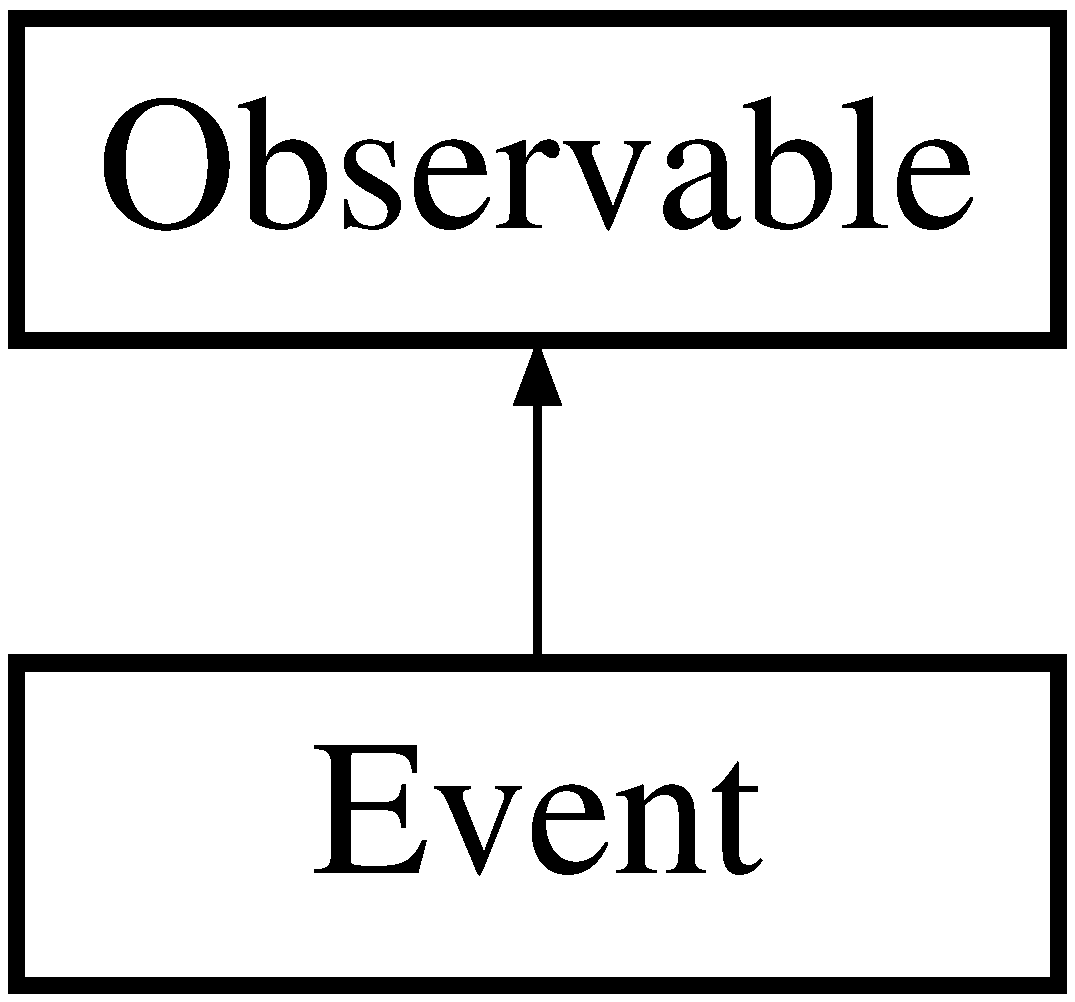
\includegraphics[height=2.000000cm]{class_event}
\end{center}
\end{figure}
\subsection*{Public Member Functions}
\begin{DoxyCompactItemize}
\item 
\hypertarget{class_event_ae136cad4600ea64e07cab62fd6a93b60}{Pcap\-Packet {\bfseries get\-Packet} ()}\label{class_event_ae136cad4600ea64e07cab62fd6a93b60}

\item 
\hypertarget{class_event_a6a2d84d2654abd587513672b8b9127db}{long {\bfseries get\-Time\-Stamp\-In\-Millis} ()}\label{class_event_a6a2d84d2654abd587513672b8b9127db}

\item 
\hypertarget{class_event_a4957820c452bcf147b8ad45be46a85d2}{Date {\bfseries get\-Time\-Stamp} ()}\label{class_event_a4957820c452bcf147b8ad45be46a85d2}

\end{DoxyCompactItemize}


The documentation for this class was generated from the following file\-:\begin{DoxyCompactItemize}
\item 
src/Event.\-java\end{DoxyCompactItemize}

\hypertarget{class_hasher}{\section{Hasher Class Reference}
\label{class_hasher}\index{Hasher@{Hasher}}
}
Inheritance diagram for Hasher\-:\begin{figure}[H]
\begin{center}
\leavevmode
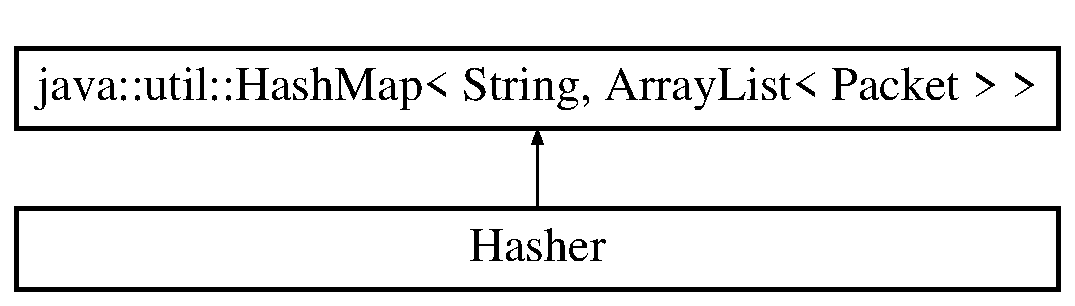
\includegraphics[height=2.000000cm]{class_hasher}
\end{center}
\end{figure}
\subsection*{Public Member Functions}
\begin{DoxyCompactItemize}
\item 
\hypertarget{class_hasher_aa9f27121ca5b6a51806eaa55ccf841f0}{void {\bfseries add} (String key, \hyperlink{class_packet}{Packet} packet)}\label{class_hasher_aa9f27121ca5b6a51806eaa55ccf841f0}

\item 
\hypertarget{class_hasher_a5a753730f82b945f0b076ce9cf9f3934}{Array\-List$<$ \hyperlink{class_packet}{Packet} $>$ {\bfseries put} (String key, Array\-List$<$ \hyperlink{class_packet}{Packet} $>$ list)}\label{class_hasher_a5a753730f82b945f0b076ce9cf9f3934}

\end{DoxyCompactItemize}


The documentation for this class was generated from the following file\-:\begin{DoxyCompactItemize}
\item 
src/Hasher.\-java\end{DoxyCompactItemize}

\hypertarget{class_packet}{\section{Packet Class Reference}
\label{class_packet}\index{Packet@{Packet}}
}
Inheritance diagram for Packet\-:\begin{figure}[H]
\begin{center}
\leavevmode
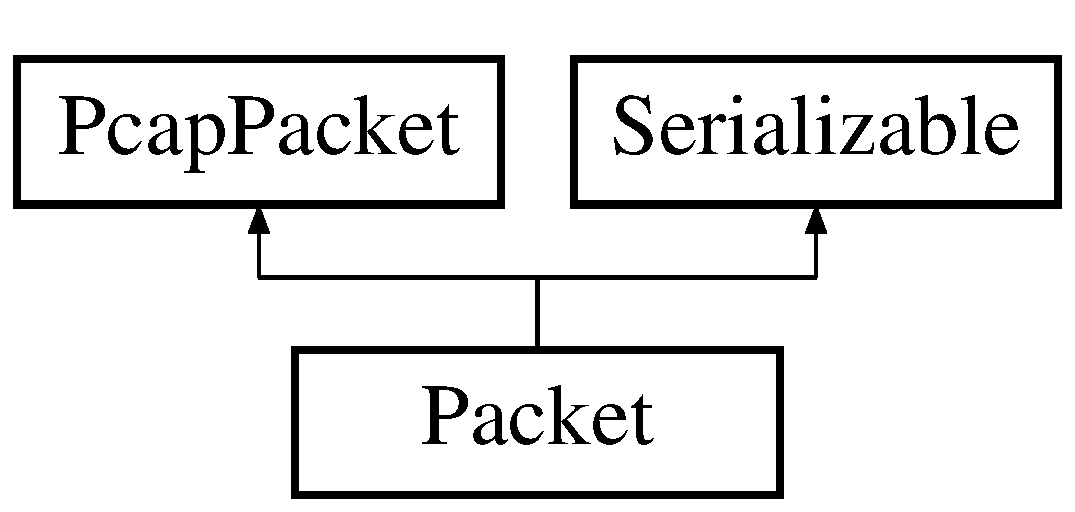
\includegraphics[height=2.000000cm]{class_packet}
\end{center}
\end{figure}


\subsection{Detailed Description}
\hyperlink{class_packet}{Packet} class extends Pcap\-Packet and implements serializable interface. It is used because Pcap\-Packet does not implement serializable.

\begin{DoxyAuthor}{Author}
amit 
\end{DoxyAuthor}


The documentation for this class was generated from the following file\-:\begin{DoxyCompactItemize}
\item 
src/Packet.\-java\end{DoxyCompactItemize}

\hypertarget{class_payload_retriever}{\section{Payload\-Retriever Class Reference}
\label{class_payload_retriever}\index{Payload\-Retriever@{Payload\-Retriever}}
}
\subsection*{Static Public Member Functions}
\begin{DoxyCompactItemize}
\item 
static byte\mbox{[}$\,$\mbox{]} \hyperlink{class_payload_retriever_aca349057334c97cd9bc1b4df3e76fb63}{get\-U\-D\-P\-Payload} (\hyperlink{class_packet}{Packet} packet)
\end{DoxyCompactItemize}


\subsection{Detailed Description}
This class implements all method used for getting udp payload from the packets captured. \begin{DoxyAuthor}{Author}
amit 
\end{DoxyAuthor}


\subsection{Member Function Documentation}
\hypertarget{class_payload_retriever_aca349057334c97cd9bc1b4df3e76fb63}{\index{Payload\-Retriever@{Payload\-Retriever}!get\-U\-D\-P\-Payload@{get\-U\-D\-P\-Payload}}
\index{get\-U\-D\-P\-Payload@{get\-U\-D\-P\-Payload}!PayloadRetriever@{Payload\-Retriever}}
\subsubsection[{get\-U\-D\-P\-Payload}]{\setlength{\rightskip}{0pt plus 5cm}static byte \mbox{[}$\,$\mbox{]} Payload\-Retriever.\-get\-U\-D\-P\-Payload (
\begin{DoxyParamCaption}
\item[{{\bf Packet}}]{packet}
\end{DoxyParamCaption}
)\hspace{0.3cm}{\ttfamily [static]}}}\label{class_payload_retriever_aca349057334c97cd9bc1b4df3e76fb63}
used to find the payload of the packet. 
\begin{DoxyParams}{Parameters}
{\em packet} & instance of \hyperlink{class_packet}{Packet} class. \\
\hline
\end{DoxyParams}
\begin{DoxyReturn}{Returns}
payload in bytes for the packet 
\end{DoxyReturn}


The documentation for this class was generated from the following file\-:\begin{DoxyCompactItemize}
\item 
src/Payload\-Retriever.\-java\end{DoxyCompactItemize}

\hypertarget{class_pcap_reader}{\section{Pcap\-Reader Class Reference}
\label{class_pcap_reader}\index{Pcap\-Reader@{Pcap\-Reader}}
}
\subsection*{Static Public Member Functions}
\begin{DoxyCompactItemize}
\item 
static Array\-List$<$ \hyperlink{class_packet}{Packet} $>$ \hyperlink{class_pcap_reader_a2b96ae4b1eeab28b808aa3bb2f6bcafd}{read\-File} (String filename, int num\-Of\-Packets)
\item 
static \hyperlink{class_packet}{Packet} \hyperlink{class_pcap_reader_a52de923b89cbe077fa30ab1fafc3d4c8}{read\-Packet} (String filename)
\item 
static \hyperlink{class_packet}{Packet} \hyperlink{class_pcap_reader_a3d07d30f780c0ecf09ab6b8d38930dbb}{read\-Packet} (String filename, int offset)
\item 
\hypertarget{class_pcap_reader_a3f57ae8d5071abdf1c3de086d2b1f892}{static void {\bfseries main} (String\mbox{[}$\,$\mbox{]} args)}\label{class_pcap_reader_a3f57ae8d5071abdf1c3de086d2b1f892}

\end{DoxyCompactItemize}


\subsection{Detailed Description}
This class holds all methods for reading packets from a Pcap file. \begin{DoxyAuthor}{Author}
amit 
\end{DoxyAuthor}


\subsection{Member Function Documentation}
\hypertarget{class_pcap_reader_a2b96ae4b1eeab28b808aa3bb2f6bcafd}{\index{Pcap\-Reader@{Pcap\-Reader}!read\-File@{read\-File}}
\index{read\-File@{read\-File}!PcapReader@{Pcap\-Reader}}
\subsubsection[{read\-File}]{\setlength{\rightskip}{0pt plus 5cm}static Array\-List$<${\bf Packet}$>$ Pcap\-Reader.\-read\-File (
\begin{DoxyParamCaption}
\item[{String}]{filename, }
\item[{int}]{num\-Of\-Packets}
\end{DoxyParamCaption}
)\hspace{0.3cm}{\ttfamily [static]}}}\label{class_pcap_reader_a2b96ae4b1eeab28b808aa3bb2f6bcafd}
This methods reads the number of packets from the given file and returns list of packets. 
\begin{DoxyParams}{Parameters}
{\em filename} & name of the pcap file \\
\hline
{\em num\-Of\-Packets} & total packets to read from the file \\
\hline
\end{DoxyParams}
\begin{DoxyReturn}{Returns}
list of packets read from the file 
\end{DoxyReturn}
\hypertarget{class_pcap_reader_a52de923b89cbe077fa30ab1fafc3d4c8}{\index{Pcap\-Reader@{Pcap\-Reader}!read\-Packet@{read\-Packet}}
\index{read\-Packet@{read\-Packet}!PcapReader@{Pcap\-Reader}}
\subsubsection[{read\-Packet}]{\setlength{\rightskip}{0pt plus 5cm}static {\bf Packet} Pcap\-Reader.\-read\-Packet (
\begin{DoxyParamCaption}
\item[{String}]{filename}
\end{DoxyParamCaption}
)\hspace{0.3cm}{\ttfamily [static]}}}\label{class_pcap_reader_a52de923b89cbe077fa30ab1fafc3d4c8}
This method is used to get a packet from the given pcap file 
\begin{DoxyParams}{Parameters}
{\em filename} & name of the pcap file \\
\hline
\end{DoxyParams}
\begin{DoxyReturn}{Returns}
The retrieved packet 
\end{DoxyReturn}
\hypertarget{class_pcap_reader_a3d07d30f780c0ecf09ab6b8d38930dbb}{\index{Pcap\-Reader@{Pcap\-Reader}!read\-Packet@{read\-Packet}}
\index{read\-Packet@{read\-Packet}!PcapReader@{Pcap\-Reader}}
\subsubsection[{read\-Packet}]{\setlength{\rightskip}{0pt plus 5cm}static {\bf Packet} Pcap\-Reader.\-read\-Packet (
\begin{DoxyParamCaption}
\item[{String}]{filename, }
\item[{int}]{offset}
\end{DoxyParamCaption}
)\hspace{0.3cm}{\ttfamily [static]}}}\label{class_pcap_reader_a3d07d30f780c0ecf09ab6b8d38930dbb}
This method reads and returns a packet from pcap file at a certain offset value in the file. 
\begin{DoxyParams}{Parameters}
{\em filename} & name of the pcap file \\
\hline
{\em offset} & offset count from the start of file \\
\hline
\end{DoxyParams}
\begin{DoxyReturn}{Returns}
packet at the given offset location. 
\end{DoxyReturn}


The documentation for this class was generated from the following file\-:\begin{DoxyCompactItemize}
\item 
src/Pcap\-Reader.\-java\end{DoxyCompactItemize}

\hypertarget{class_protocol_state_machine}{\section{Protocol\-State\-Machine Class Reference}
\label{class_protocol_state_machine}\index{Protocol\-State\-Machine@{Protocol\-State\-Machine}}
}
\subsection*{Static Public Member Functions}
\begin{DoxyCompactItemize}
\item 
static boolean \hyperlink{class_protocol_state_machine_ab16976efe8017a6cf4b7bac29fa6a5bd}{is\-Time\-Out} (long timer, long time)
\item 
static void \hyperlink{class_protocol_state_machine_ab210fe7d2c2a4ce4c4120cdb70b8b6fd}{set\-Current\-Packet} (\hyperlink{class_packet}{Packet} packet)
\item 
static void \hyperlink{class_protocol_state_machine_af033fb0f497cbf5c1c3e006fb09cf966}{main} (String\mbox{[}$\,$\mbox{]} args)
\end{DoxyCompactItemize}


\subsection{Detailed Description}
Contains fields for objects \hyperlink{class_state}{State} Machine, \hyperlink{class_transition}{Transition}, \hyperlink{class_packet}{Packet} and Connection. \begin{DoxyAuthor}{Author}
amit 
\end{DoxyAuthor}


\subsection{Member Function Documentation}
\hypertarget{class_protocol_state_machine_ab16976efe8017a6cf4b7bac29fa6a5bd}{\index{Protocol\-State\-Machine@{Protocol\-State\-Machine}!is\-Time\-Out@{is\-Time\-Out}}
\index{is\-Time\-Out@{is\-Time\-Out}!ProtocolStateMachine@{Protocol\-State\-Machine}}
\subsubsection[{is\-Time\-Out}]{\setlength{\rightskip}{0pt plus 5cm}static boolean Protocol\-State\-Machine.\-is\-Time\-Out (
\begin{DoxyParamCaption}
\item[{long}]{timer, }
\item[{long}]{time}
\end{DoxyParamCaption}
)\hspace{0.3cm}{\ttfamily [static]}}}\label{class_protocol_state_machine_ab16976efe8017a6cf4b7bac29fa6a5bd}
checks whether the process has exceeded time limit 
\begin{DoxyParams}{Parameters}
{\em timer} & \\
\hline
{\em time} & \\
\hline
\end{DoxyParams}
\begin{DoxyReturn}{Returns}
true if time exceeds timeout else false 
\end{DoxyReturn}
\hypertarget{class_protocol_state_machine_af033fb0f497cbf5c1c3e006fb09cf966}{\index{Protocol\-State\-Machine@{Protocol\-State\-Machine}!main@{main}}
\index{main@{main}!ProtocolStateMachine@{Protocol\-State\-Machine}}
\subsubsection[{main}]{\setlength{\rightskip}{0pt plus 5cm}static void Protocol\-State\-Machine.\-main (
\begin{DoxyParamCaption}
\item[{String\mbox{[}$\,$\mbox{]}}]{args}
\end{DoxyParamCaption}
)\hspace{0.3cm}{\ttfamily [static]}}}\label{class_protocol_state_machine_af033fb0f497cbf5c1c3e006fb09cf966}
main method for the program 
\begin{DoxyParams}{Parameters}
{\em args} & array of strings as command line arguments \\
\hline
\end{DoxyParams}
(psm.\-S\-M.\-get\-Current\-State().equals(psm.\-S\-M.\-get\-End\-State())) \hypertarget{class_protocol_state_machine_ab210fe7d2c2a4ce4c4120cdb70b8b6fd}{\index{Protocol\-State\-Machine@{Protocol\-State\-Machine}!set\-Current\-Packet@{set\-Current\-Packet}}
\index{set\-Current\-Packet@{set\-Current\-Packet}!ProtocolStateMachine@{Protocol\-State\-Machine}}
\subsubsection[{set\-Current\-Packet}]{\setlength{\rightskip}{0pt plus 5cm}static void Protocol\-State\-Machine.\-set\-Current\-Packet (
\begin{DoxyParamCaption}
\item[{{\bf Packet}}]{packet}
\end{DoxyParamCaption}
)\hspace{0.3cm}{\ttfamily [static]}}}\label{class_protocol_state_machine_ab210fe7d2c2a4ce4c4120cdb70b8b6fd}
setter for \hyperlink{class_packet}{Packet} field 
\begin{DoxyParams}{Parameters}
{\em instance} & of class \hyperlink{class_packet}{Packet} \\
\hline
\end{DoxyParams}


The documentation for this class was generated from the following file\-:\begin{DoxyCompactItemize}
\item 
src/Protocol\-State\-Machine.\-java\end{DoxyCompactItemize}

\hypertarget{class_state}{\section{State Class Reference}
\label{class_state}\index{State@{State}}
}
\subsection*{Public Member Functions}
\begin{DoxyCompactItemize}
\item 
String \hyperlink{class_state_a2366ee1a7f1f44c75588c282520b7f1f}{get\-Name} ()
\item 
void \hyperlink{class_state_a84f6bf30ca26f93109f8b61e6a661ccb}{set\-Name} (String name)
\item 
void \hyperlink{class_state_aa909e96de36cd52f36e451eb223a8abc}{add\-Entry\-Action} (Method entry)
\item 
void \hyperlink{class_state_a3243408f4e2b54aa84738e285cf6f400}{add\-Exit\-Action} (Method exit)
\item 
void \hyperlink{class_state_ab8224460e24ecc6d6bd77f895d98aba1}{add\-Transitions} (Method transitions)
\end{DoxyCompactItemize}
\subsection*{Public Attributes}
\begin{DoxyCompactItemize}
\item 
\hypertarget{class_state_aa4ad4ae247532abaee49cb794e25ba57}{Method {\bfseries on\-Entry}}\label{class_state_aa4ad4ae247532abaee49cb794e25ba57}

\item 
\hypertarget{class_state_a2c6bcf1d0e84499ff2a95f0ce7d6face}{Method {\bfseries on\-Exit}}\label{class_state_a2c6bcf1d0e84499ff2a95f0ce7d6face}

\item 
\hypertarget{class_state_adc3230770759c25d37100af107aec281}{Method {\bfseries next\-State}}\label{class_state_adc3230770759c25d37100af107aec281}

\end{DoxyCompactItemize}


\subsection{Detailed Description}
This class describes the entry, exit and next state of each transition state during the course of program \begin{DoxyAuthor}{Author}
amit 
\end{DoxyAuthor}


\subsection{Member Function Documentation}
\hypertarget{class_state_aa909e96de36cd52f36e451eb223a8abc}{\index{State@{State}!add\-Entry\-Action@{add\-Entry\-Action}}
\index{add\-Entry\-Action@{add\-Entry\-Action}!State@{State}}
\subsubsection[{add\-Entry\-Action}]{\setlength{\rightskip}{0pt plus 5cm}void State.\-add\-Entry\-Action (
\begin{DoxyParamCaption}
\item[{Method}]{entry}
\end{DoxyParamCaption}
)}}\label{class_state_aa909e96de36cd52f36e451eb223a8abc}
setter for entry method for this state 
\begin{DoxyParams}{Parameters}
{\em entry} & entry method for this state \\
\hline
\end{DoxyParams}
\hypertarget{class_state_a3243408f4e2b54aa84738e285cf6f400}{\index{State@{State}!add\-Exit\-Action@{add\-Exit\-Action}}
\index{add\-Exit\-Action@{add\-Exit\-Action}!State@{State}}
\subsubsection[{add\-Exit\-Action}]{\setlength{\rightskip}{0pt plus 5cm}void State.\-add\-Exit\-Action (
\begin{DoxyParamCaption}
\item[{Method}]{exit}
\end{DoxyParamCaption}
)}}\label{class_state_a3243408f4e2b54aa84738e285cf6f400}
setter for exit method for this state 
\begin{DoxyParams}{Parameters}
{\em exit} & exit method for this state \\
\hline
\end{DoxyParams}
\hypertarget{class_state_ab8224460e24ecc6d6bd77f895d98aba1}{\index{State@{State}!add\-Transitions@{add\-Transitions}}
\index{add\-Transitions@{add\-Transitions}!State@{State}}
\subsubsection[{add\-Transitions}]{\setlength{\rightskip}{0pt plus 5cm}void State.\-add\-Transitions (
\begin{DoxyParamCaption}
\item[{Method}]{transitions}
\end{DoxyParamCaption}
)}}\label{class_state_ab8224460e24ecc6d6bd77f895d98aba1}
setter for transition method for this state 
\begin{DoxyParams}{Parameters}
{\em transitions} & next method for the current state \\
\hline
\end{DoxyParams}
\hypertarget{class_state_a2366ee1a7f1f44c75588c282520b7f1f}{\index{State@{State}!get\-Name@{get\-Name}}
\index{get\-Name@{get\-Name}!State@{State}}
\subsubsection[{get\-Name}]{\setlength{\rightskip}{0pt plus 5cm}String State.\-get\-Name (
\begin{DoxyParamCaption}
{}
\end{DoxyParamCaption}
)}}\label{class_state_a2366ee1a7f1f44c75588c282520b7f1f}
getter for name of the state \begin{DoxyReturn}{Returns}
name of state 
\end{DoxyReturn}
\hypertarget{class_state_a84f6bf30ca26f93109f8b61e6a661ccb}{\index{State@{State}!set\-Name@{set\-Name}}
\index{set\-Name@{set\-Name}!State@{State}}
\subsubsection[{set\-Name}]{\setlength{\rightskip}{0pt plus 5cm}void State.\-set\-Name (
\begin{DoxyParamCaption}
\item[{String}]{name}
\end{DoxyParamCaption}
)}}\label{class_state_a84f6bf30ca26f93109f8b61e6a661ccb}
setter for name of the state 
\begin{DoxyParams}{Parameters}
{\em name} & name of the state \\
\hline
\end{DoxyParams}


The documentation for this class was generated from the following file\-:\begin{DoxyCompactItemize}
\item 
src/State.\-java\end{DoxyCompactItemize}

\hypertarget{class_state_machine}{\section{State\-Machine Class Reference}
\label{class_state_machine}\index{State\-Machine@{State\-Machine}}
}
Inheritance diagram for State\-Machine\-:\begin{figure}[H]
\begin{center}
\leavevmode
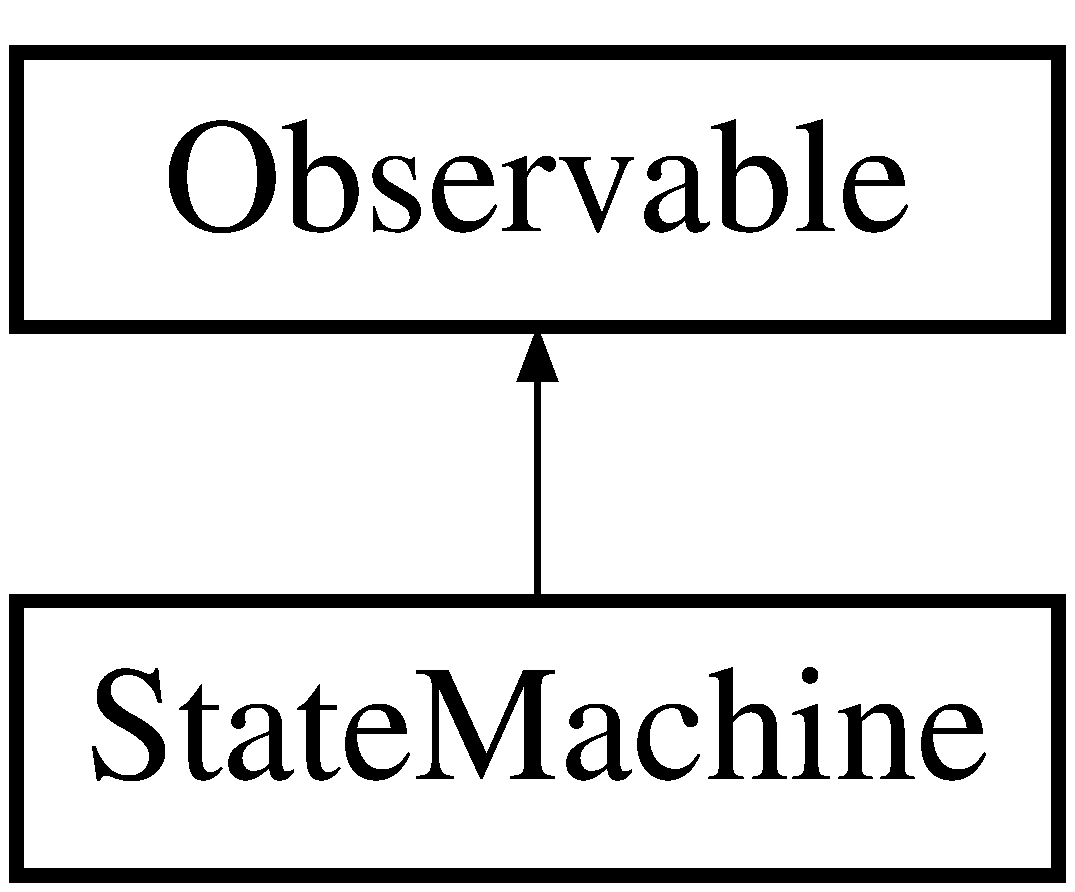
\includegraphics[height=2.000000cm]{class_state_machine}
\end{center}
\end{figure}
\subsection*{Public Member Functions}
\begin{DoxyCompactItemize}
\item 
void \hyperlink{class_state_machine_ad7ef0f4c2c7390eba41096b57025299c}{set\-Current\-State} (\hyperlink{class_transition_support}{Transition\-Support} t)
\item 
\hyperlink{class_state}{State} \hyperlink{class_state_machine_a31dc2fcca3fb09e8b004b9d21b7c6aa5}{get\-Initial\-State} ()
\item 
\hyperlink{class_state}{State} \hyperlink{class_state_machine_a8ec03fd0f1350838b05ea8765d0f012a}{get\-End\-State} ()
\item 
int \hyperlink{class_state_machine_a97dc1b3bc38a8d046035ef52dc8b2621}{get\-Numberof\-States} ()
\item 
\hyperlink{class_state}{State} \hyperlink{class_state_machine_afb2aab31dddcbefe3d4cb9eb5fdef61f}{get\-State} (String name)
\item 
\hyperlink{class_state}{State} \hyperlink{class_state_machine_adfe7ca2ef6ac4763ad49fde662564ec1}{get\-Current\-State} ()
\end{DoxyCompactItemize}


\subsection{Detailed Description}
Class that stores initial state, current state, end state, all transition states and total number of possible states \begin{DoxyAuthor}{Author}
amit 
\end{DoxyAuthor}


\subsection{Member Function Documentation}
\hypertarget{class_state_machine_adfe7ca2ef6ac4763ad49fde662564ec1}{\index{State\-Machine@{State\-Machine}!get\-Current\-State@{get\-Current\-State}}
\index{get\-Current\-State@{get\-Current\-State}!StateMachine@{State\-Machine}}
\subsubsection[{get\-Current\-State}]{\setlength{\rightskip}{0pt plus 5cm}{\bf State} State\-Machine.\-get\-Current\-State (
\begin{DoxyParamCaption}
{}
\end{DoxyParamCaption}
)}}\label{class_state_machine_adfe7ca2ef6ac4763ad49fde662564ec1}
getter for current state \begin{DoxyReturn}{Returns}
current state of the state machine. 
\end{DoxyReturn}
\hypertarget{class_state_machine_a8ec03fd0f1350838b05ea8765d0f012a}{\index{State\-Machine@{State\-Machine}!get\-End\-State@{get\-End\-State}}
\index{get\-End\-State@{get\-End\-State}!StateMachine@{State\-Machine}}
\subsubsection[{get\-End\-State}]{\setlength{\rightskip}{0pt plus 5cm}{\bf State} State\-Machine.\-get\-End\-State (
\begin{DoxyParamCaption}
{}
\end{DoxyParamCaption}
)}}\label{class_state_machine_a8ec03fd0f1350838b05ea8765d0f012a}
getter for end state. \begin{DoxyReturn}{Returns}
end state for this state machine 
\end{DoxyReturn}
\hypertarget{class_state_machine_a31dc2fcca3fb09e8b004b9d21b7c6aa5}{\index{State\-Machine@{State\-Machine}!get\-Initial\-State@{get\-Initial\-State}}
\index{get\-Initial\-State@{get\-Initial\-State}!StateMachine@{State\-Machine}}
\subsubsection[{get\-Initial\-State}]{\setlength{\rightskip}{0pt plus 5cm}{\bf State} State\-Machine.\-get\-Initial\-State (
\begin{DoxyParamCaption}
{}
\end{DoxyParamCaption}
)}}\label{class_state_machine_a31dc2fcca3fb09e8b004b9d21b7c6aa5}
getter for initial state. \begin{DoxyReturn}{Returns}
initial state of this state machine 
\end{DoxyReturn}
\hypertarget{class_state_machine_a97dc1b3bc38a8d046035ef52dc8b2621}{\index{State\-Machine@{State\-Machine}!get\-Numberof\-States@{get\-Numberof\-States}}
\index{get\-Numberof\-States@{get\-Numberof\-States}!StateMachine@{State\-Machine}}
\subsubsection[{get\-Numberof\-States}]{\setlength{\rightskip}{0pt plus 5cm}int State\-Machine.\-get\-Numberof\-States (
\begin{DoxyParamCaption}
{}
\end{DoxyParamCaption}
)}}\label{class_state_machine_a97dc1b3bc38a8d046035ef52dc8b2621}
getter for total number of states for this state machine \begin{DoxyReturn}{Returns}
total number of states 
\end{DoxyReturn}
\hypertarget{class_state_machine_afb2aab31dddcbefe3d4cb9eb5fdef61f}{\index{State\-Machine@{State\-Machine}!get\-State@{get\-State}}
\index{get\-State@{get\-State}!StateMachine@{State\-Machine}}
\subsubsection[{get\-State}]{\setlength{\rightskip}{0pt plus 5cm}{\bf State} State\-Machine.\-get\-State (
\begin{DoxyParamCaption}
\item[{String}]{name}
\end{DoxyParamCaption}
)}}\label{class_state_machine_afb2aab31dddcbefe3d4cb9eb5fdef61f}
getter for a particular state according to state name 
\begin{DoxyParams}{Parameters}
{\em name} & name of the state to get \\
\hline
\end{DoxyParams}
\begin{DoxyReturn}{Returns}
state as per name in parameter 
\end{DoxyReturn}
\hypertarget{class_state_machine_ad7ef0f4c2c7390eba41096b57025299c}{\index{State\-Machine@{State\-Machine}!set\-Current\-State@{set\-Current\-State}}
\index{set\-Current\-State@{set\-Current\-State}!StateMachine@{State\-Machine}}
\subsubsection[{set\-Current\-State}]{\setlength{\rightskip}{0pt plus 5cm}void State\-Machine.\-set\-Current\-State (
\begin{DoxyParamCaption}
\item[{{\bf Transition\-Support}}]{t}
\end{DoxyParamCaption}
)}}\label{class_state_machine_ad7ef0f4c2c7390eba41096b57025299c}
setter for current state. This method also notifies observers about the change in state. 
\begin{DoxyParams}{Parameters}
{\em t} & \\
\hline
\end{DoxyParams}


The documentation for this class was generated from the following file\-:\begin{DoxyCompactItemize}
\item 
src/State\-Machine.\-java\end{DoxyCompactItemize}

\hypertarget{class_transition}{\section{Transition Class Reference}
\label{class_transition}\index{Transition@{Transition}}
}
Inheritance diagram for Transition\-:\begin{figure}[H]
\begin{center}
\leavevmode
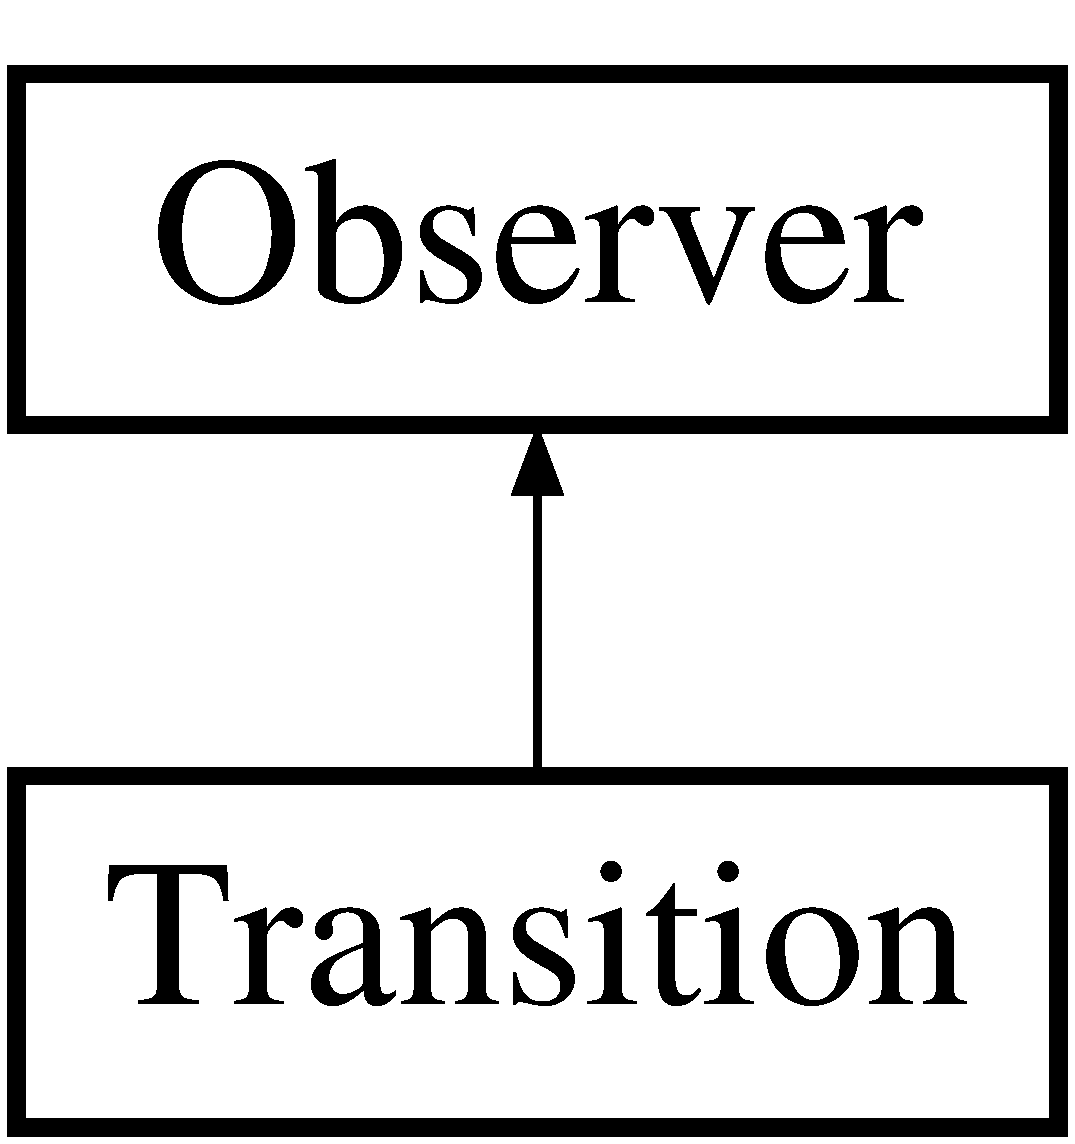
\includegraphics[height=2.000000cm]{class_transition}
\end{center}
\end{figure}
\subsection*{Public Member Functions}
\begin{DoxyCompactItemize}
\item 
\hypertarget{class_transition_acee1af44b7d58aa1c02976738dcfaf80}{\hyperlink{class_state}{State} {\bfseries getfrom\-State} ()}\label{class_transition_acee1af44b7d58aa1c02976738dcfaf80}

\item 
\hypertarget{class_transition_a11d7374ead7d8114485507b77925b797}{\hyperlink{class_state}{State} {\bfseries getto\-State} ()}\label{class_transition_a11d7374ead7d8114485507b77925b797}

\item 
\hypertarget{class_transition_ad22714a1e7afd83b110191669f6447f9}{void {\bfseries update} (Observable o, Object obj)}\label{class_transition_ad22714a1e7afd83b110191669f6447f9}

\end{DoxyCompactItemize}


The documentation for this class was generated from the following file\-:\begin{DoxyCompactItemize}
\item 
src/Transition.\-java\end{DoxyCompactItemize}

\hypertarget{class_transition_support}{\section{Transition\-Support Class Reference}
\label{class_transition_support}\index{Transition\-Support@{Transition\-Support}}
}
\subsection*{Public Member Functions}
\begin{DoxyCompactItemize}
\item 
void \hyperlink{class_transition_support_a7b69faa809da771794eb7293cb444f9c}{set\-Arguments} (int exp, int enp, Object...\-parameters)
\item 
\hyperlink{class_state}{State} \hyperlink{class_transition_support_a0a9f0d558c6f6e9024c0384a7f831e4f}{get\-Start\-State} ()
\item 
\hyperlink{class_state}{State} \hyperlink{class_transition_support_a6c0772c22388fe100e92588ac2734469}{get\-End\-State} ()
\item 
Object \hyperlink{class_transition_support_a420f5aff45ea69e01190c45288f7e7a4}{get\-Calling\-Object} ()
\item 
Object\mbox{[}$\,$\mbox{]} \hyperlink{class_transition_support_a3ce6e760ca114f388edd663b650f87f0}{getfrom\-Arguments} ()
\item 
Object\mbox{[}$\,$\mbox{]} \hyperlink{class_transition_support_a99189bbaa88a9cc76597b71b4145f31d}{getto\-Arguments} ()
\item 
Object\mbox{[}$\,$\mbox{]} \hyperlink{class_transition_support_a8985efe149e070d9f43e17c9d9384b1b}{get\-Arguments} ()
\end{DoxyCompactItemize}


\subsection{Member Function Documentation}
\hypertarget{class_transition_support_a8985efe149e070d9f43e17c9d9384b1b}{\index{Transition\-Support@{Transition\-Support}!get\-Arguments@{get\-Arguments}}
\index{get\-Arguments@{get\-Arguments}!TransitionSupport@{Transition\-Support}}
\subsubsection[{get\-Arguments}]{\setlength{\rightskip}{0pt plus 5cm}Object \mbox{[}$\,$\mbox{]} Transition\-Support.\-get\-Arguments (
\begin{DoxyParamCaption}
{}
\end{DoxyParamCaption}
)}}\label{class_transition_support_a8985efe149e070d9f43e17c9d9384b1b}
getter for parameters only \begin{DoxyReturn}{Returns}
array of arguments 
\end{DoxyReturn}
\hypertarget{class_transition_support_a420f5aff45ea69e01190c45288f7e7a4}{\index{Transition\-Support@{Transition\-Support}!get\-Calling\-Object@{get\-Calling\-Object}}
\index{get\-Calling\-Object@{get\-Calling\-Object}!TransitionSupport@{Transition\-Support}}
\subsubsection[{get\-Calling\-Object}]{\setlength{\rightskip}{0pt plus 5cm}Object Transition\-Support.\-get\-Calling\-Object (
\begin{DoxyParamCaption}
{}
\end{DoxyParamCaption}
)}}\label{class_transition_support_a420f5aff45ea69e01190c45288f7e7a4}
getter for calling object \begin{DoxyReturn}{Returns}
calling object for transition 
\end{DoxyReturn}
\hypertarget{class_transition_support_a6c0772c22388fe100e92588ac2734469}{\index{Transition\-Support@{Transition\-Support}!get\-End\-State@{get\-End\-State}}
\index{get\-End\-State@{get\-End\-State}!TransitionSupport@{Transition\-Support}}
\subsubsection[{get\-End\-State}]{\setlength{\rightskip}{0pt plus 5cm}{\bf State} Transition\-Support.\-get\-End\-State (
\begin{DoxyParamCaption}
{}
\end{DoxyParamCaption}
)}}\label{class_transition_support_a6c0772c22388fe100e92588ac2734469}
getter for to state \begin{DoxyReturn}{Returns}
to state for transition 
\end{DoxyReturn}
\hypertarget{class_transition_support_a3ce6e760ca114f388edd663b650f87f0}{\index{Transition\-Support@{Transition\-Support}!getfrom\-Arguments@{getfrom\-Arguments}}
\index{getfrom\-Arguments@{getfrom\-Arguments}!TransitionSupport@{Transition\-Support}}
\subsubsection[{getfrom\-Arguments}]{\setlength{\rightskip}{0pt plus 5cm}Object \mbox{[}$\,$\mbox{]} Transition\-Support.\-getfrom\-Arguments (
\begin{DoxyParamCaption}
{}
\end{DoxyParamCaption}
)}}\label{class_transition_support_a3ce6e760ca114f388edd663b650f87f0}
getter for parameters and from argument \begin{DoxyReturn}{Returns}
array of arguments 
\end{DoxyReturn}
\hypertarget{class_transition_support_a0a9f0d558c6f6e9024c0384a7f831e4f}{\index{Transition\-Support@{Transition\-Support}!get\-Start\-State@{get\-Start\-State}}
\index{get\-Start\-State@{get\-Start\-State}!TransitionSupport@{Transition\-Support}}
\subsubsection[{get\-Start\-State}]{\setlength{\rightskip}{0pt plus 5cm}{\bf State} Transition\-Support.\-get\-Start\-State (
\begin{DoxyParamCaption}
{}
\end{DoxyParamCaption}
)}}\label{class_transition_support_a0a9f0d558c6f6e9024c0384a7f831e4f}
getter for from state \begin{DoxyReturn}{Returns}
from state for the transition 
\end{DoxyReturn}
\hypertarget{class_transition_support_a99189bbaa88a9cc76597b71b4145f31d}{\index{Transition\-Support@{Transition\-Support}!getto\-Arguments@{getto\-Arguments}}
\index{getto\-Arguments@{getto\-Arguments}!TransitionSupport@{Transition\-Support}}
\subsubsection[{getto\-Arguments}]{\setlength{\rightskip}{0pt plus 5cm}Object \mbox{[}$\,$\mbox{]} Transition\-Support.\-getto\-Arguments (
\begin{DoxyParamCaption}
{}
\end{DoxyParamCaption}
)}}\label{class_transition_support_a99189bbaa88a9cc76597b71b4145f31d}
getter for parameters and to argument \begin{DoxyReturn}{Returns}
array of arguments 
\end{DoxyReturn}
\hypertarget{class_transition_support_a7b69faa809da771794eb7293cb444f9c}{\index{Transition\-Support@{Transition\-Support}!set\-Arguments@{set\-Arguments}}
\index{set\-Arguments@{set\-Arguments}!TransitionSupport@{Transition\-Support}}
\subsubsection[{set\-Arguments}]{\setlength{\rightskip}{0pt plus 5cm}void Transition\-Support.\-set\-Arguments (
\begin{DoxyParamCaption}
\item[{int}]{exp, }
\item[{int}]{enp, }
\item[{Object...}]{parameters}
\end{DoxyParamCaption}
)}}\label{class_transition_support_a7b69faa809da771794eb7293cb444f9c}
sets entry parameter, exit parameter and other parameters for the class 
\begin{DoxyParams}{Parameters}
{\em exp} & exit parameter for the class \\
\hline
{\em enp} & entry parameter for the class \\
\hline
{\em parameters} & object parameters \\
\hline
\end{DoxyParams}


The documentation for this class was generated from the following file\-:\begin{DoxyCompactItemize}
\item 
src/Transition\-Support.\-java\end{DoxyCompactItemize}

%--- End generated contents ---

% Index
\newpage
\phantomsection
\addcontentsline{toc}{chapter}{Index}
\printindex

\end{document}
